\section{Kiến thức nền tảng và nghiên cứu liên quan}

Chương này trình bày các kiến thức cần thiết để xây dựng hệ thống UAV tự động hạ cánh bằng thị giác máy tính, gắp hàng và cất cánh trở lại. Nội dung được sắp xếp theo chuỗi xử lý của hệ thống: mô hình UAV, camera, phát hiện ArUco, ước lượng pose, điều khiển, giao tiếp với PX4 và cơ cấu gripper.

\subsection{Tổng quan về UAV }

UAV quadrotor là phương tiện bay sử dụng bốn cụm động 
cơ - cánh quạt để tạo lực nâng và điều khiển chuyển 
động. Bốn rotor thường được bố trí theo hình chữ X 
hoặc hình dấu cộng trên cùng một mặt phẳng. 
Mô hình uav S500 mà đồ án sử dụng là dạng chữ X.

\begin{figure}[H]
  \centering
  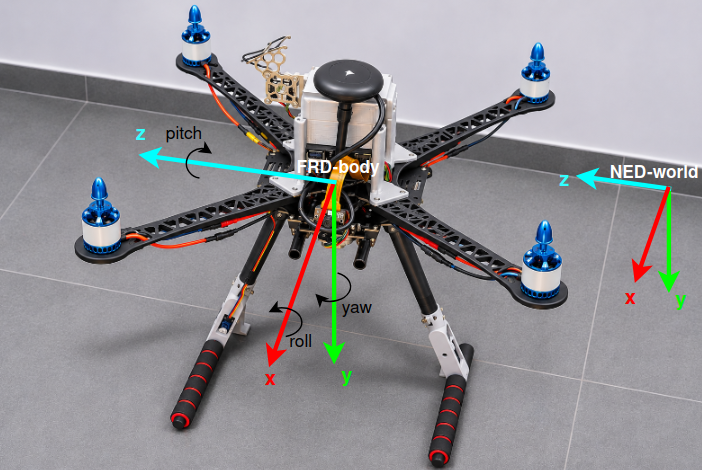
\includegraphics[width=0.6\textwidth]{images/02-uav-model-and-coordinate.png}
  \caption{Mô hình UAV S500 và hệ trục tọa độ liên quan.}
  \label{fig:model-and-coordinate-uav}
\end{figure}

Hình \ref{fig:model-and-coordinate-uav} mô tả hệ trục body của UAV được chọn theo FRD-front\_right\_down và hệ trục world được chọn theo NED-north\_east\_down. Hai rotor quay theo chiều kim đồng hồ và hai 
rotor quay ngược chiều kim đồng hồ nhằm triệt 
tiêu mô-men phản lực tổng cộng khi UAV bay ổn định.

Hình \ref{fig:nguyen-ly-dieu-khien-uav} minh họa nguyên lý điều khiển chuyển động của UAV quadrotor thông qua việc thay đổi tốc độ quay của bốn rotor.
\begin{figure}[H]
  \centering
  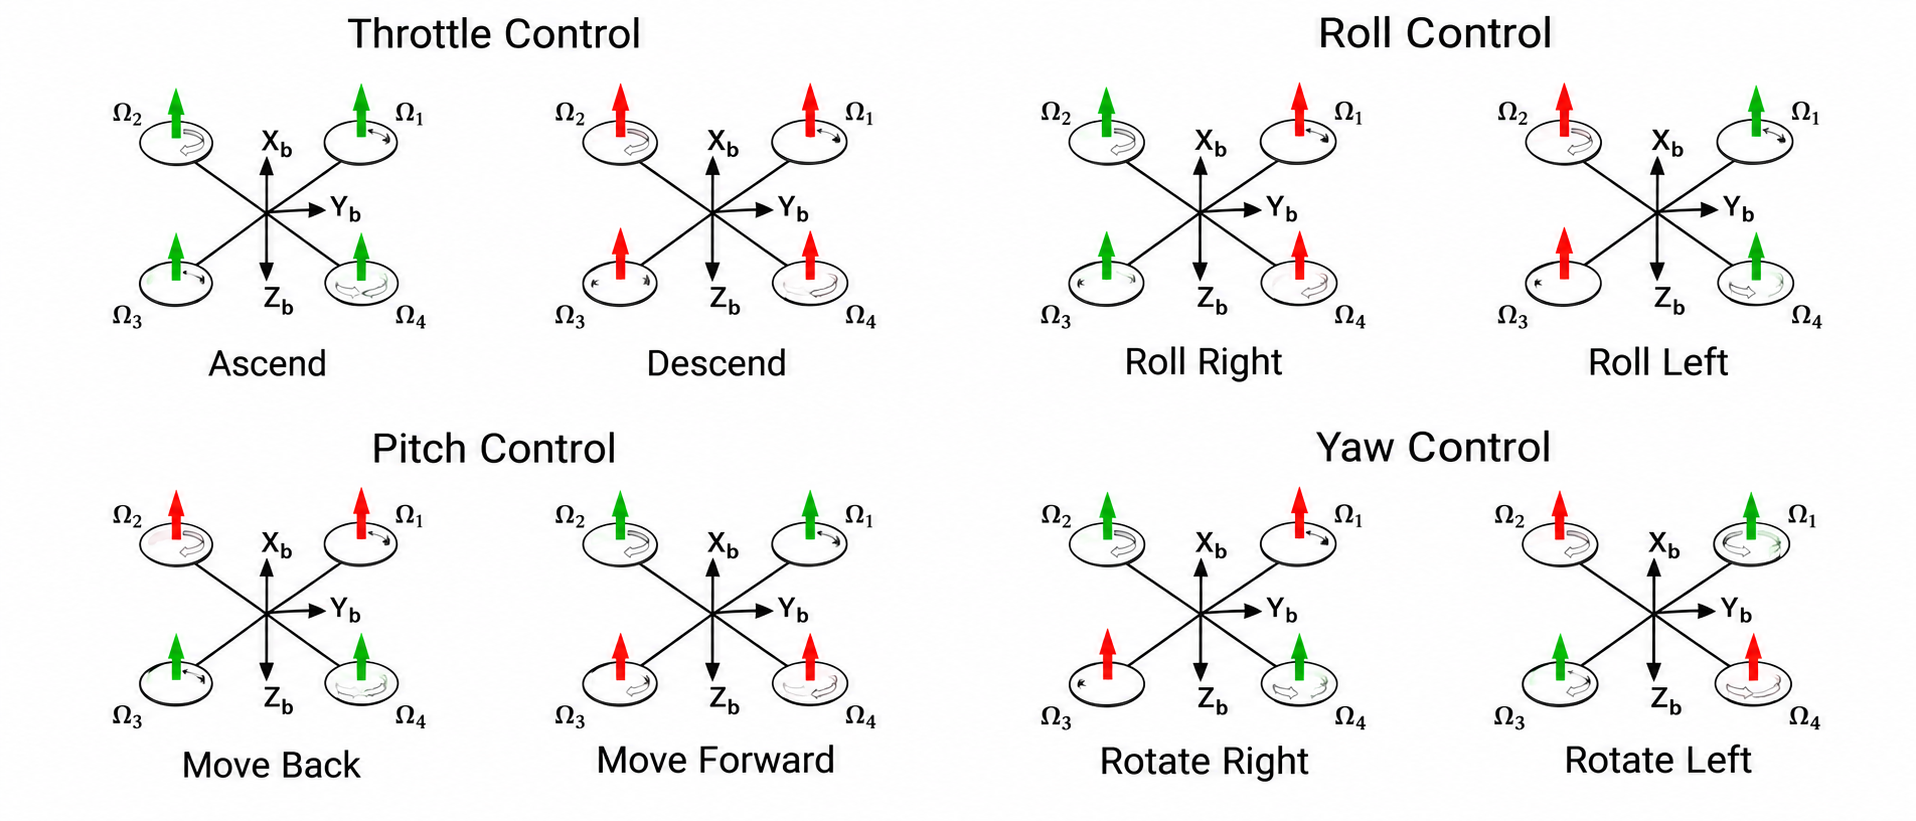
\includegraphics[width=1.0\textwidth]{images/02-propeller-direction.png}
  \caption{Nguyên lý điều khiển độ cao và các chuyển động Roll, Pitch, Yaw của UAV quadrotor.}
  \label{fig:nguyen-ly-dieu-khien-uav}
\end{figure}

Khi tốc độ quay của các rotor tăng hoặc giảm đồng thời, tổng lực nâng thay đổi, giúp UAV điều chỉnh độ cao. Bên cạnh đó, sự chênh lệch lực nâng giữa các rotor tạo ra mô-men điều khiển chuyển động Roll và Pitch, trong khi sự chênh lệch mô-men phản lực giữa các cặp rotor quay ngược chiều tạo ra chuyển động Yaw.

Trong bài toán hạ cánh, 
chuyển động theo phương ngang được sử dụng để đưa 
tâm UAV về phía trên tâm marker, trong khi chuyển 
động theo phương đứng được sử dụng để giảm độ cao. 
Sai số yaw cũng cần được xem xét vì hướng của UAV 
ảnh hưởng đến phép biến đổi giữa hệ tọa độ camera, 
thân UAV và hệ tọa độ world.

\subsection{Mã ArUco}
ArUco (Augmented Reality University of Cordoba) là một loại mã đánh dấu thị giác (fiducial marker) được sử dụng phổ biến trong các hệ thống thị giác máy tính nhằm nhận dạng và xác định vị trí tương đối của đối tượng thông qua hình ảnh thu nhận từ camera. Mã ArUco được phát triển dưới dạng các hình vuông chứa những ô nhị phân màu đen và trắng, cho phép hệ thống nhận dạng từng mã thông qua một bộ từ điển được định nghĩa trước
\subsubsection{Cấu trúc và từ điển mã ArUco}

\textbf{a)} ArUco là một mã có dạng hình vuông, gồm đường viền đen và một ma trận bit nhị phân ở bên trong. 
Đường biên màu đen giúp phát hiện marker nhanh hơn vì nó tương phản với môi trường xung quanh, 
bằng các thuật toán thị giác máy tính cơ bản (như tạo ngưỡng phân đoạn - thresholding, hay tìm đường viền - contour extraction) có thể ngay lập tức phát hiện ra hình vuông đen này với tốc độ cực nhanh (real-time). Máy tính chỉ việc tìm ra 4 góc của viền đen là đã hoàn thành xong bước xác định vị trí.

Sau đó việc mã hóa nhị phân phần bên trong cho phép nhận dạng ID cũng như áp dụng các kỹ thuật phát hiện và sửa lỗi. 

Hình \ref{fig:vi-du-anh-marker} minh họa một ví dụ về ảnh marker ArUco. 
\begin{figure}[H]
  \centering
  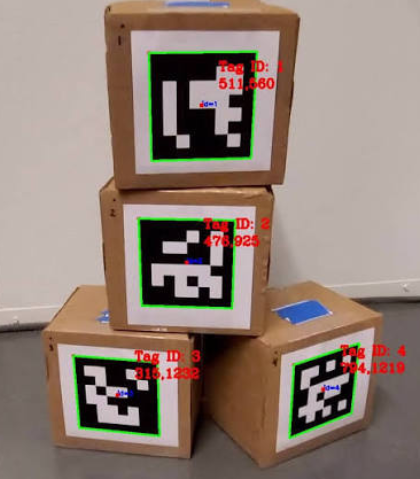
\includegraphics[width=0.3\textwidth]{images/02-aruco-ex.png}
  \caption{Ví dụ về ảnh marker}
  \label{fig:vi-du-anh-marker}
\end{figure}

Kích thước của marker được quyết định bởi ma trận bên trong, ví dụ marker size 4x4 được tạo thành từ 16 bits.
Marker còn xác định chính xác góc quay gốc của nó trong môi trường, 
đảm bảo các góc được nhận diện một cách duy nhất và không sai lệch.

\textbf{b)} Từ điển mã ArUco là tập các mã ArUco dùng trong các ứng dụng cụ thể, đơn giản là một tập mã hóa nhị phân của mỗi marker.

Hai đặc tính của mã ArUco:
\begin{itemize}
  \item Kích thước từ điển là số lượng marker chứa trong nó
  \item Kích thước marker là số lượng bit nhị phân trong ma trận bên trong của marker
\end{itemize}
ID marker không phải giá trị thập phân chuyển từ binary qua, vì marker size lớn
sẽ tạo các số lớn phi thực tế, do đó ID marker là index của marker trong từ điển. 
Ví dụ 5 marker đầu là ID 0,1,2,3,4.
\subsubsection{Nguyên lý nhận diện mã ArUco}
\begin{figure}[H]
  \centering
  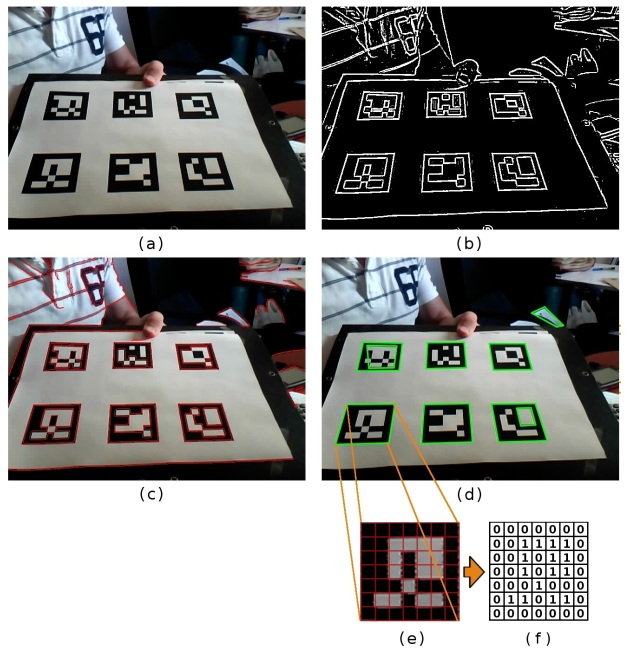
\includegraphics[width=0.6\textwidth]{images/02-image-process-aruco.png}
  \caption{Quy trình phát hiện marker ArUco trong ảnh 
  (a) Original Image. 
  (b) Result of applying local thresholding. 
  (c) Contour detection. 
  (d) Polygonal approximation and removal of irrelevant contours. 
  (e) Example of marker after perspective transformation. 
  (f) Bit assignment for each cell.}
  \label{fig:tu-dong-phat-hien-marker}
\end{figure}
Hình \ref{fig:tu-dong-phat-hien-marker} minh họa quy trình phát hiện marker ArUco trong ảnh. Quy trình này bao gồm các bước chính:
\begin{enumerate}
  \item \textbf{Phân đoạn ảnh:} ảnh từ camera được chuyển sang ảnh mức xám, sau đó áp dụng local adaptive
thresholding để tạo ảnh nhị phân. 
Cách xử lý này làm nổi bật vùng sáng - tối và giúp hệ thống hoạt động tốt hơn khi độ sáng không đồng đều.
  \item \textbf{Trích xuất và lọc đường viền:} từ ảnh nhị phân, hệ thống tìm các đường viền và lần lượt loại bỏ những vùng không có đặc trưng hình học của mã ArUco. Quá trình này gồm các tiểu bước sau:
  \begin{enumerate}[a)]
    \item Trích xuất đường viền: thuật toán Suzuki--Abe được sử dụng để tìm đường biên của các vùng liên thông trên ảnh nhị phân. Kết quả ban đầu có thể chứa nhiều đường viền không liên quan, chẳng hạn đường biên của vật thể hoặc hoa văn trong môi trường.
    \item Xấp xỉ đa giác: thuật toán Douglas--Peucker đơn giản hóa mỗi đường viền thành một đa giác có ít đỉnh hơn nhưng vẫn bảo toàn hình dạng chính.
    \item Lọc tứ giác: do mã ArUco có dạng hình vuông, chỉ những đa giác lồi có bốn đỉnh và thỏa mãn các điều kiện về kích thước, khoảng cách giữa các đỉnh mới được giữ lại làm ứng viên.
    \item Loại bỏ ứng viên trùng hoặc lồng nhau:
     các đường viền quá gần nhau hoặc cùng biểu 
     diễn một vùng marker được loại bỏ nhằm 
     tránh phát hiện lặp. Sau bước này, hệ 
     thống thu được tập các vùng tứ giác ứng viên để tiếp tục giải mã.
  \end{enumerate}
  \item \textbf{Trích xuất mã nhị phân:} mỗi vùng tứ giác ứng viên được chuẩn hóa và chuyển thành một ma trận bit để phục vụ quá trình nhận dạng. Quá trình này gồm các tiểu bước sau:
  \begin{enumerate}[a)]
    \item Nắn phẳng ảnh bằng phép biến đổi phối cảnh: khi camera quan sát marker ở góc nghiêng, hình vuông có thể bị biến dạng thành hình thang hoặc hình tứ giác. Từ bốn góc đã phát hiện, hệ thống tính ma trận homography và ánh xạ vùng ứng viên về một hình vuông chuẩn nhìn trực diện.
    \item Nhị phân hóa bằng phương pháp Otsu: ảnh marker đã chuẩn hóa được chuyển thành ảnh đen--trắng. Phương pháp Otsu tự động chọn ngưỡng nhằm cực đại hóa sự phân tách giữa hai lớp điểm ảnh sáng và tối, nhờ đó hạn chế ảnh hưởng của bóng đổ hoặc độ sáng không đồng đều trong vùng marker.
    \item Chia lưới và xác định giá trị bit: vùng ảnh được chia thành một lưới tương ứng với số ô dữ liệu và phần viền của marker. Trong mỗi ô, số điểm ảnh đen và trắng được thống kê; giá trị chiếm đa số quyết định bit $0$ hoặc $1$. Kết quả là một ma trận nhị phân biểu diễn nội dung marker.
    \item Kiểm tra viền đen: các ô thuộc đường viền ngoài của mã ArUco phải có màu đen. Ứng viên sẽ bị loại nếu số bit viền sai vượt quá ngưỡng cho phép; nhờ đó, các vùng tứ giác ngẫu nhiên trong môi trường được loại bỏ trước khi so sánh với từ điển.
  \end{enumerate}
  \item \textbf{Nhận dạng và hiệu chỉnh lỗi:} ma trận bit được so sánh với các mẫu trong từ điển ArUco ở bốn hướng xoay. Khoảng cách Hamming được dùng để chọn ID phù hợp và cho phép hiệu chỉnh một số bit lỗi trong giới hạn của từ điển.
  \item \textbf{Xác định các góc marker:} sau khi nhận dạng thành công, thuật toán trả về ID và tọa độ bốn góc của marker; các tọa độ này có thể được tinh chỉnh để nâng cao độ chính xác.
\end{enumerate}

Kết quả nhận diện gồm ID và bốn điểm góc trên mặt phẳng ảnh. Từ các dữ liệu này, hệ thống xác định tâm marker; khi kết hợp với kích thước thật của marker và thông số hiệu chuẩn camera, hệ thống có thể ước lượng vị trí và tư thế tương đối bằng phương pháp PnP. Trong bài toán hạ cánh tự động, pose của marker được dùng để tính sai lệch vị trí và cung cấp tín hiệu phản hồi cho bộ điều khiển UAV.

\subsection{Camera và hiệu chuẩn}

Camera đơn cung cấp ảnh màu từ môi trường xung quanh. Trong đề tài này, camera được lắp hướng xuống để quan sát bãi đáp và marker trong quá trình tiếp cận, căn chỉnh và hạ cánh. Chất lượng của phép ước lượng pose phụ thuộc vào độ phân giải, trường nhìn, độ méo ống kính, độ rung và góc lắp camera.

\subsubsection{Mô hình camera lỗ kim}

Với mô hình camera lỗ kim, một điểm trong hệ tọa độ camera được chiếu lên mặt phẳng ảnh thông qua ma trận nội tại:
\begin{equation}
  \mathbf{K}=\begin{bmatrix}f_x & 0 & c_x\\ 0 & f_y & c_y\\ 0 & 0 & 1\end{bmatrix},
\end{equation}
trong đó $f_x$ và $f_y$ là tiêu cự theo hai phương ảnh, còn $(c_x,c_y)$ là tọa độ tâm ảnh. Với điểm không gian $\mathbf{P}_c=[X_c,Y_c,Z_c]^T$, tọa độ ảnh lý tưởng được xác định bởi:
\begin{equation}
  s\begin{bmatrix}u\\v\\1\end{bmatrix}=\mathbf{K}\begin{bmatrix}X_c\\Y_c\\Z_c\end{bmatrix},
\end{equation}
trong đó $(u,v)$ là tọa độ điểm ảnh và $s$ là hệ số tỉ lệ.

Ống kính thực tế gây ra méo xuyên tâm và méo tiếp tuyến. Vì vậy, ma trận nội tại và các hệ số méo cần được xác định trước khi dùng ảnh để ước lượng pose marker.

\subsubsection{Quy trình hiệu chuẩn}

Quy trình hiệu chuẩn camera gồm các bước chính:
\begin{enumerate}
  \item In bàn cờ hoặc bảng chuẩn có kích thước ô đã biết.
  \item Chụp nhiều ảnh ở các vị trí, khoảng cách và góc nghiêng khác nhau.
  \item Phát hiện các góc của bàn cờ trong từng ảnh.
  \item Tối ưu ma trận nội tại và hệ số méo dựa trên các điểm tương ứng.
  \item Đánh giá sai số chiếu lại và lưu thông số hiệu chuẩn để sử dụng trong chương trình xử lý ảnh.
\end{enumerate}

Camera cần được cố định chắc chắn sau khi hiệu chuẩn. Nếu vị trí hoặc góc lắp camera thay đổi, phép biến đổi giữa hệ camera và hệ thân UAV phải được xác định lại.

% TODO: Chèn ảnh bàn cờ ở nhiều góc và ảnh so sánh trước/sau hiệu chỉnh méo.
\noindent\textit{[Hình cần chèn: Bộ ảnh hiệu chuẩn camera và kết quả hiệu chỉnh méo.]}\par\vspace{18mm}
\subsection{Các hệ tọa độ}

Trong hệ thống UAV hạ cánh tự động dựa trên thị giác máy tính, việc xác định vị trí tương đối giữa UAV và mã ArUco đòi hỏi phải thống nhất quy ước các hệ tọa độ. Các hệ tọa độ được sử dụng bao gồm:

\begin{itemize}
    \item \textbf{Hệ tọa độ dẫn đường $\{N\}$ (NED):}
    Là hệ tọa độ tham chiếu cục bộ được sử dụng trong PX4, có các trục $X_N$, $Y_N$, $Z_N$ lần lượt hướng về phía Bắc (North), Đông (East) và xuống dưới (Down). Hệ này được sử dụng để biểu diễn vị trí, vận tốc và quỹ đạo chuyển động của UAV.

    \item \textbf{Hệ tọa độ thân UAV $\{B\}$ (Body frame):}
    Gắn với thân UAV và tuân theo quy ước FRD (Forward--Right--Down) của PX4. Trục $X_B$ hướng về phía trước UAV, trục $Y_B$ hướng sang phải và trục $Z_B$ hướng xuống dưới. Hệ tọa độ này được sử dụng để mô tả tư thế và chuyển động của UAV tương đối với thân máy bay.

    \item \textbf{Hệ tọa độ camera $\{C\}$ (Camera optical frame):}
    Có gốc tại tâm quang học của camera. Theo quy ước OpenCV, trục $X_C$ hướng sang phải ảnh, trục $Y_C$ hướng xuống dưới ảnh và trục $Z_C$ trùng với trục quang học, hướng từ camera về phía đối tượng quan sát.

    \item \textbf{Hệ tọa độ ảnh $\{I\}$ (Image frame):}
    Là hệ tọa độ hai chiều trên mặt phẳng ảnh, có gốc tại góc trên bên trái. Trục $u$ hướng sang phải và trục $v$ hướng xuống dưới. Tọa độ điểm ảnh được biểu diễn bởi $(u,v)$, với đơn vị pixel.

    \item \textbf{Hệ tọa độ marker $\{M\}$ (Marker frame):}
    Có gốc tại tâm mã ArUco. Theo quy ước mặc định của OpenCV, hai trục $X_M$ và $Y_M$ nằm trong mặt phẳng marker, lần lượt hướng sang phải và lên trên theo chiều chuẩn của mã, trong khi $Z_M$ vuông góc với mặt phẳng marker và hướng ra khỏi mặt in.
\end{itemize}

Mối quan hệ giữa hai hệ tọa độ bất kỳ được biểu diễn thông qua ma trận biến đổi đồng nhất:

\begin{equation}
    {}^{A}\mathbf{T}_{B} =
    \begin{bmatrix}
        {}^{A}\mathbf{R}_{B} & {}^{A}\mathbf{t}_{B} \\
        \mathbf{0}^{T} & 1
    \end{bmatrix},
    \label{eq:homogeneous_transform}
\end{equation}

trong đó ${}^{A}\mathbf{R}_{B}\in SO(3)$ là ma trận quay mô tả hướng của hệ $B$ so với hệ $A$, và ${}^{A}\mathbf{t}_{B}\in\mathbb{R}^{3}$ là vector tịnh tiến biểu diễn vị trí gốc hệ $B$ trong hệ $A$.
\begin{figure}[H]
  \centering
  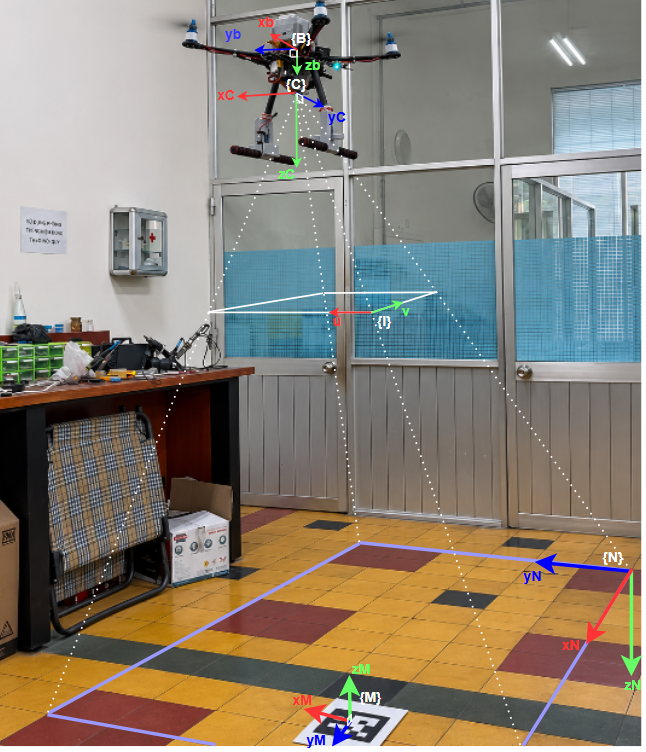
\includegraphics[width=0.8\textwidth]{images/03-all-coordinate.png}
  \caption{Các hệ trục tọa độ}
  \label{fig:all-coordinate}
\end{figure}
Hình \ref{fig:all-coordinate} minh họa các hệ trục tọa độ được sử dụng trong hệ thống.
Đối với hệ thống đang xét, phép biến đổi từ hệ tọa độ marker sang hệ tọa độ dẫn đường được biểu diễn bởi:

\begin{equation}
    {}^{N}\mathbf{T}_{M}
    =
    {}^{N}\mathbf{T}_{B}
    {}^{B}\mathbf{T}_{C}
    {}^{C}\mathbf{T}_{M},
    \label{eq:coordinate_transform_chain}
\end{equation}
\indent trong đó ${}^{C}\mathbf{T}_{M}$ được xác định thông qua quá trình nhận diện và ước lượng tư thế ArUco, ${}^{B}\mathbf{T}_{C}$ phụ thuộc vào vị trí và hướng lắp đặt camera trên UAV, còn ${}^{N}\mathbf{T}_{B}$ mô tả tư thế của UAV trong hệ tọa độ dẫn đường.

\subsection{Ước lượng pose bằng PnP}

Sau khi phát hiện mã ArUco, thuật toán nhận diện cung cấp ID và tọa độ bốn góc marker trên mặt phẳng ảnh. Để xác định vị trí và hướng của marker trong không gian ba chiều, hệ thống sử dụng bài toán Perspective-n-Point (PnP), dựa trên mối quan hệ giữa các điểm 3D đã biết trên marker và các điểm 2D tương ứng được quan sát bởi camera.

\begin{figure}[H]
  \centering
  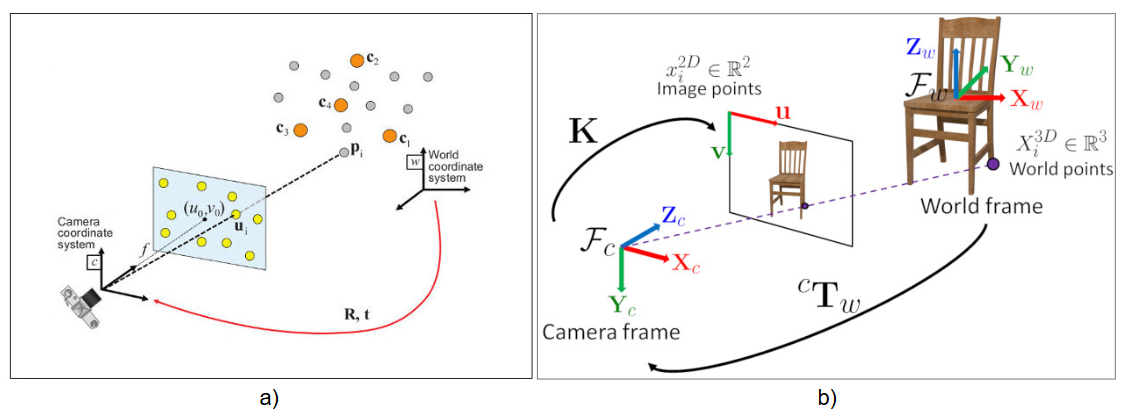
\includegraphics[width=1\textwidth]{images/03-PnP.png}
  \caption{(a) Phép chiếu phối cảnh từ không gian 3D lên
    mặt phẳng ảnh 2D;
    (b) Phép biến đổi tọa độ và phép chiếu phối cảnh
    thông qua mô hình camera.}
  \label{fig:PnP}
\end{figure}
Quá trình ước lượng tư thế bằng PnP được minh họa trong
Hình~\ref{fig:PnP}. Trong đó, Hình~\ref{fig:PnP}(a)
biểu diễn mô hình phép chiếu phối cảnh từ không gian ba chiều
xuống mặt phẳng ảnh hai chiều. Một điểm 3D được biến đổi
từ hệ tọa độ tham chiếu sang hệ tọa độ camera thông qua
ma trận quay $\mathbf{R}$ và vector tịnh tiến $\mathbf{t}$,
sau đó được chiếu lên mặt phẳng ảnh theo mô hình camera
lỗ kim với ma trận nội tại $\mathbf{K}$.

Hình~\ref{fig:PnP}(b) minh họa chi tiết hai bước
biến đổi hình học: (1) chuyển tọa độ điểm 3D từ hệ tham
chiếu sang hệ camera thông qua ma trận biến đổi đồng nhất;
(2) chiếu điểm 3D trong hệ camera lên mặt phẳng ảnh để
thu được tọa độ pixel $(u,v)$. Thông qua các cặp điểm
tương ứng 3D--2D, bài toán PnP cho phép ước lượng tư thế
tương đối gồm sáu bậc tự do (6-DoF), bao gồm ba thành
phần tịnh tiến và ba thành phần quay.

Trong bài toán nhận diện ArUco, hệ tọa độ tham chiếu
được thay bằng hệ tọa độ marker $\{M\}$. Các điểm 3D
là bốn góc của marker với kích thước đã biết, trong khi
các điểm 2D tương ứng được xác định thông qua thuật
toán phát hiện ArUco trên ảnh camera. Kết quả PnP cung
cấp phép biến đổi ${}^{C}\mathbf{T}_{M}$, mô tả vị trí
và hướng của marker trong hệ tọa độ camera.

Theo mô hình camera lỗ kim, quan hệ phép chiếu được biểu diễn bởi:

\begin{equation}
    s_i \tilde{\mathbf{p}}_i
    =
    \mathbf{K}
    \left(
        {}^{C}\mathbf{R}_{M}\mathbf{P}_i
        +
        {}^{C}\mathbf{t}_{M}
    \right),
    \label{eq:pnp_projection}
\end{equation}
\indent trong đó:
\begin{itemize}
    \item $\mathbf{P}_i=[X_i,Y_i,Z_i]^T$ là tọa độ điểm thứ $i$ trong hệ marker.
    \item $\tilde{\mathbf{p}}_i=[u_i,v_i,1]^T$ là tọa độ thuần nhất của điểm ảnh tương ứng sau khi hiệu chỉnh méo.
    \item $\mathbf{K}$ là ma trận thông số nội tại của camera.
    \item ${}^{C}\mathbf{R}_{M}$ và ${}^{C}\mathbf{t}_{M}$ lần lượt là ma trận quay và vector tịnh tiến của hệ marker so với hệ camera.
    \item $s_i$ là hệ số tỷ lệ của phép chiếu phối cảnh.
\end{itemize}

Ma trận nội tại camera được biểu diễn dưới dạng:

\begin{equation}
    \mathbf{K} =
    \begin{bmatrix}
        f_x & 0 & c_x \\
        0 & f_y & c_y \\
        0 & 0 & 1
    \end{bmatrix},
    \label{eq:camera_intrinsic}
\end{equation}

trong đó $f_x$, $f_y$ là tiêu cự biểu diễn theo đơn vị pixel, còn $(c_x,c_y)$ là tọa độ điểm chính ảnh.

Với mã ArUco hình vuông có chiều dài cạnh $L$, gốc tọa độ được đặt tại tâm marker. Theo quy ước được sử dụng, tọa độ bốn góc trong hệ marker lần lượt là:

\begin{equation}
\begin{aligned}
    \mathbf{P}_1 &= [-L/2,\; L/2,\; 0]^T,\\
    \mathbf{P}_2 &= [ L/2,\; L/2,\; 0]^T,\\
    \mathbf{P}_3 &= [ L/2,\;-L/2,\; 0]^T,\\
    \mathbf{P}_4 &= [-L/2,\;-L/2,\; 0]^T.
\end{aligned}
\label{eq:marker_corners}
\end{equation}

Từ các cặp điểm tương ứng 3D--2D, thuật toán PnP ước lượng phép quay và phép tịnh tiến sao cho sai số chiếu lại giữa các điểm ảnh dự đoán và quan sát được là nhỏ nhất. Trong quá trình này, các tham số hiệu chuẩn camera và hệ số méo ống kính được sử dụng để nâng cao độ chính xác của phép ước lượng.

Kết quả ước lượng gồm vector quay $\mathbf{rvec}$ và vector tịnh tiến $\mathbf{tvec}$. Vector quay được chuyển thành ma trận quay thông qua công thức Rodrigues, trong khi vector tịnh tiến biểu diễn vị trí tâm marker trong hệ tọa độ camera:

\begin{equation}
    {}^{C}\mathbf{t}_{M}
    =
    \begin{bmatrix}
        x_C\\y_C\\z_C
    \end{bmatrix}.
    \label{eq:aruco_translation}
\end{equation}

Trong trường hợp camera hướng xuống mặt đất, thành phần $z_C$ biểu diễn khoảng cách theo trục quang học từ camera đến mặt phẳng marker. Hai thành phần $x_C$ và $y_C$ mô tả độ lệch vị trí tương đối của marker theo các trục camera.

Để phục vụ quá trình điều khiển hạ cánh, tọa độ marker được chuyển từ hệ camera sang hệ thân UAV theo:

\begin{equation}
    {}^{B}\mathbf{p}_{M}
    =
    {}^{B}\mathbf{R}_{C}
    {}^{C}\mathbf{t}_{M}
    +
    {}^{B}\mathbf{t}_{C},
    \label{eq:camera_to_body}
\end{equation}

trong đó ${}^{B}\mathbf{R}_{C}$ mô tả hướng lắp đặt camera và ${}^{B}\mathbf{t}_{C}$ biểu diễn vị trí tâm camera so với gốc tọa độ thân UAV.

Thông qua phép biến đổi này, sai lệch vị trí giữa UAV và marker được xác định trong hệ tọa độ thân, làm cơ sở xây dựng tín hiệu điều khiển chuyển động ngang và giảm độ cao trong quá trình hạ cánh tự động.


\subsection{Điều khiển PID và visual servoing}

Visual servoing là phương pháp sử dụng thông tin thu được từ camera làm tín hiệu phản hồi cho bộ điều khiển. Trong bài toán này, các sai số thị giác được tạo từ pose của marker và được dùng để điều khiển vận tốc hoặc vị trí đặt của UAV.

Với sai số $e(t)$ và tín hiệu điều khiển $u(t)$, bộ điều khiển PID có dạng:
\begin{equation}
  u(t)=K_p e(t)+K_i\int_0^t e(\tau)\,d\tau+K_d\frac{de(t)}{dt}.
\end{equation}
Trong đó, thành phần tỉ lệ tạo phản ứng theo sai số hiện tại, thành phần tích phân loại bỏ sai số tĩnh và thành phần vi phân giúp giảm dao động khi sai số thay đổi nhanh. Đối với UAV, các thành phần điều khiển có thể được thiết kế riêng cho sai số ngang, độ cao và góc yaw.

Một chu trình hạ cánh có thể được chia thành các giai đoạn:
\begin{enumerate}
  \item \textbf{Tìm marker:} UAV di chuyển đến vùng mà marker có thể xuất hiện trong trường nhìn.
  \item \textbf{Căn chỉnh ngang:} giữ độ cao tương đối ổn định và giảm sai số vị trí trên mặt phẳng bãi đáp.
  \item \textbf{Hạ độ cao:} khi sai số ngang đủ nhỏ và marker được phát hiện ổn định, UAV giảm độ cao theo giới hạn an toàn.
  \item \textbf{Xác nhận hạ cánh:} kiểm tra độ cao, vận tốc và thời gian ổn định trước khi kích hoạt gripper.
\end{enumerate}

Khi dữ liệu marker bị mất, hệ thống không nên tiếp tục điều khiển dựa trên dữ liệu cũ vô hạn. Cần đặt thời gian timeout, giới hạn vận tốc và trạng thái dừng hoặc bay lên lại để giảm nguy cơ va chạm. Bộ điều khiển cũng cần có giới hạn tích phân để tránh hiện tượng tích lũy sai số khi UAV chưa nhìn thấy marker.

% TODO: Chèn sơ đồ khối vòng điều khiển hạ cánh.
\noindent\textit{[Hình cần chèn: Camera/ArUco $\rightarrow$ sai số pose $\rightarrow$ PID $\rightarrow$ setpoint UAV $\rightarrow$ PX4.]}\par\vspace{18mm}

\subsection{PX4, ROS 2 và chế độ Offboard}

PX4 là firmware điều khiển bay đảm nhiệm các chức năng ổn định attitude, điều khiển vị trí và quản lý trạng thái bay. Raspberry Pi 5 chạy các node ROS 2 để thu nhận ảnh, xử lý ArUco, tính toán pose và tạo lệnh điều khiển cấp cao.

Trong cấu hình đề xuất, các thành phần chính gồm:
\begin{itemize}
  \item \textbf{Camera node:} thu ảnh và công bố dữ liệu hình ảnh.
  \item \textbf{ArUco node:} phát hiện marker, ước lượng pose và công bố kết quả.
  \item \textbf{Landing controller node:} tính sai số, chạy PID và tạo setpoint vận tốc hoặc vị trí.
  \item \textbf{Mission/state machine node:} quản lý các trạng thái tìm marker, hạ cánh, gắp hàng và cất cánh.
  \item \textbf{Gripper node:} phát lệnh servo và nhận trạng thái xác nhận cơ cấu gắp.
  \item \textbf{PX4 flight controller:} nhận setpoint, ổn định UAV và gửi trạng thái bay về máy tính đồng hành.
\end{itemize}

Giao tiếp giữa ROS 2 và PX4 có thể được thực hiện qua uXRCE-DDS. Ở chế độ Offboard, máy tính đồng hành gửi liên tục các setpoint và tín hiệu duy trì chế độ điều khiển. Trước khi chuyển sang Offboard, hệ thống cần kiểm tra kết nối, trạng thái định vị, nguồn pin, trạng thái arm và tần số gửi setpoint. Nếu mất kết nối hoặc không còn setpoint hợp lệ, PX4 phải chuyển sang hành vi an toàn được cấu hình trước.

% TODO: Chèn sơ đồ node ROS 2 và đường truyền dữ liệu tới PX4.
\noindent\textit{[Hình cần chèn: Kiến trúc ROS 2--uXRCE-DDS--PX4--UAV.]}\par\vspace{18mm}

\subsection{Cơ cấu gripper}

Cơ cấu gripper có nhiệm vụ giữ kiện hàng trong quá trình UAV cất cánh và bay. Khi thiết kế gripper, cần xem xét khối lượng cơ cấu, tải trọng 1 kg, kích thước kiện hàng, hành trình đóng mở, lực giữ và vị trí lắp đặt trên thân UAV.

Việc treo tải bên dưới UAV làm thay đổi vị trí trọng tâm và mô-men quán tính của hệ thống. Vì vậy, cơ cấu cần được lắp chắc chắn, hạn chế dao động của kiện hàng và không che khuất camera. Khối lượng của gripper và kiện hàng cũng phải nằm trong khả năng tạo lực nâng của bốn rotor.

Servo có thể được điều khiển bằng góc quay hoặc độ rộng xung PWM. Máy trạng thái không nên chỉ dựa vào lệnh đóng servo để kết luận gắp thành công; cần có điều kiện xác nhận, chẳng hạn như vị trí servo, công tắc hành trình, cảm biến lực hoặc kiểm tra tải sau khi UAV bắt đầu cất cánh. Nếu không có cảm biến riêng, hệ thống có thể sử dụng một khoảng thời gian giữ và kiểm tra trạng thái ổn định của UAV, đồng thời ghi nhận đây là một giới hạn của thiết kế.

% TODO: Chèn bản vẽ CAD hoặc ảnh thực tế của gripper.
\noindent\textit{[Hình cần chèn: Cơ cấu gripper, vị trí lắp trên UAV và trạng thái mở/đóng.]}\par\vspace{18mm}

\subsection{Máy trạng thái Landing--Pickup--Takeoff}

Máy trạng thái giúp chia nhiệm vụ phức tạp thành các trạng thái có điều kiện chuyển rõ ràng. Một phiên bản cơ bản có thể gồm:
\begin{enumerate}
  \item \textbf{SEARCH\_MARKER:} tìm marker trong ảnh và giữ UAV ở vùng an toàn.
  \item \textbf{ALIGN:} điều chỉnh vị trí ngang và hướng của UAV so với marker.
  \item \textbf{DESCEND:} hạ độ cao khi marker được phát hiện ổn định và sai số nằm trong giới hạn.
  \item \textbf{LANDED:} xác nhận UAV đã tiếp xúc hoặc đã ổn định trên bãi đáp.
  \item \textbf{GRAB:} đóng gripper và kiểm tra điều kiện gắp.
  \item \textbf{TAKEOFF:} tăng độ cao đến mức an toàn và tiếp tục nhiệm vụ.
  \item \textbf{ABORT/FAILSAFE:} dừng, bay lên hoặc chuyển sang điều khiển thủ công khi mất marker, mất kết nối hoặc phát hiện điều kiện không an toàn.
\end{enumerate}

Mỗi trạng thái cần quy định rõ điều kiện vào, điều kiện thoát, timeout và hành vi khi lỗi. Cách tổ chức này giúp tránh việc các node điều khiển gửi lệnh mâu thuẫn, đồng thời tạo log rõ ràng để phân tích khi thử nghiệm thất bại.

% TODO: Chèn sơ đồ máy trạng thái toàn bộ nhiệm vụ.
\noindent\textit{[Hình cần chèn: SEARCH--ALIGN--DESCEND--LANDED--GRAB--TAKEOFF và nhánh ABORT.]}\par\vspace{18mm}

\subsection{Các công trình liên quan}

Các nghiên cứu về hạ cánh UAV bằng thị giác thường tập trung vào ba nội dung: thiết kế marker có thể nhận dạng ở nhiều khoảng cách, ước lượng pose tương đối từ camera đơn và xây dựng bộ điều khiển dựa trên thông tin thị giác. Một số công trình sử dụng một marker duy nhất, trong khi các công trình khác sử dụng marker nhiều lớp hoặc nhiều kích thước để duy trì khả năng nhận dạng khi UAV thay đổi độ cao.

Một hướng phổ biến là dùng các góc của ArUco marker kết hợp với thông số hiệu chuẩn camera để giải bài toán PnP. Pose thu được được đưa vào bộ điều khiển PID hoặc bộ điều khiển visual servoing nhằm giảm sai số ngang trước khi hạ độ cao. Các kết quả nghiên cứu cho thấy độ chính xác không chỉ phụ thuộc vào thuật toán điều khiển mà còn phụ thuộc mạnh vào kích thước marker, trường nhìn camera, độ trễ xử lý, ánh sáng và rung động của UAV.

Trong các hệ thống giao hàng, ngoài bài toán hạ cánh còn có bài toán giữ và thả kiện hàng. Cơ cấu gripper phải nhẹ, đủ lực giữ và không làm mất ổn định UAV. Một số hệ thống bổ sung cảm biến để xác nhận đã gắp được vật thể; các hệ thống đơn giản hơn sử dụng máy trạng thái và điều kiện thời gian để điều phối servo.

So với các công trình chỉ xét hạ cánh hoặc chỉ xét cơ cấu gắp, đồ án này hướng đến việc tích hợp cả hai nhiệm vụ trên cùng một nền tảng Raspberry Pi 5, ROS 2 và PX4. Trọng tâm của đồ án là xây dựng một quy trình có thể kiểm thử từng module và đánh giá định lượng toàn bộ chuỗi hạ cánh--gắp hàng--cất cánh.

% TODO: Bổ sung bảng so sánh các công trình liên quan.
% Nên có các cột: tài liệu, loại marker, camera, nền tảng bay,
% phương pháp điều khiển, có gắp hàng hay không, mô phỏng/thực nghiệm.
\begin{table}[H]
  \centering
  \caption{Gợi ý bảng so sánh các công trình liên quan}
  \label{tab:so-sanh-cong-trinh}
  \begin{tabularx}{\textwidth}{|>{\raggedright\arraybackslash}p{3.0cm}|>{\raggedright\arraybackslash}p{2.5cm}|>{\raggedright\arraybackslash}p{2.4cm}|>{\raggedright\arraybackslash}X|}
    \hline
    \textbf{Công trình} & \textbf{Marker/cảm biến} & \textbf{Điều khiển} & \textbf{Phạm vi đánh giá}\\
    \hline
    Công trình 1 & Bổ sung sau & Bổ sung sau & Bổ sung sau\\
    \hline
    Công trình 2 & Bổ sung sau & Bổ sung sau & Bổ sung sau\\
    \hline
    Đồ án này & ArUco + camera đơn & PID + máy trạng thái & Hạ cánh, gắp hàng, cất cánh\\
    \hline
  \end{tabularx}
\end{table}

\subsection{Tóm tắt chương}

Chương này đã trình bày các cơ sở về UAV quadrotor, hệ tọa độ, camera, hiệu chuẩn, phát hiện ArUco, ước lượng pose bằng PnP, điều khiển PID, visual servoing, PX4, ROS 2, Offboard và cơ cấu gripper. Đây là cơ sở để xây dựng kiến trúc phần mềm, thuật toán điều khiển và quy trình thực nghiệm ở các chương tiếp theo.
